\documentclass{beamer}

\usepackage[utf8]{inputenc}
\usepackage[T1]{fontenc}
\usepackage{amsmath}
\usepackage{graphicx}

\usetheme{Madrid}
\usecolortheme{crane}


\title{NROR - 1. Domača naloga}
\author{Jure Križman, 23211023}
\date{\today}





\begin{document}

\begin{frame}
\titlepage
\centering

\includegraphics[width=0.25\textwidth]{sliak3.png}
\end{frame}


\section{Predstavitev uporabljene metode}
\begin{frame}
\tableofcontents[currentsection] % Ukaz za vstavljanje kazala
\end{frame}
\begin{frame}
\begin{itemize}
\item Za iskanje $\pi$ z uporabo Monte Carlo metode, predstavljamo kvadrat s stranico 2 enoti in vanj vpišemo krog s polmerom 1 enoto.
\pause
\item Generiramo veliko naključnih točk znotraj kvadrata.
\pause
\item Izračunamo razmerje med točkami, ki so znotraj kroga, in celotnim številom točk.
\item To razmerje pomnožimo s 4, da dobimo približek za $\pi$: $\pi \approx \frac{\text{Točke v krogu}}{\text{Skupno število točk}} \times 4$
\end{itemize}
\end{frame}




\section{Prikaz grafa naključnih točk}
\begin{frame}
\tableofcontents[currentsection] % Ukaz za vstavljanje kazala
\end{frame}
\begin{frame}
\begin{figure}
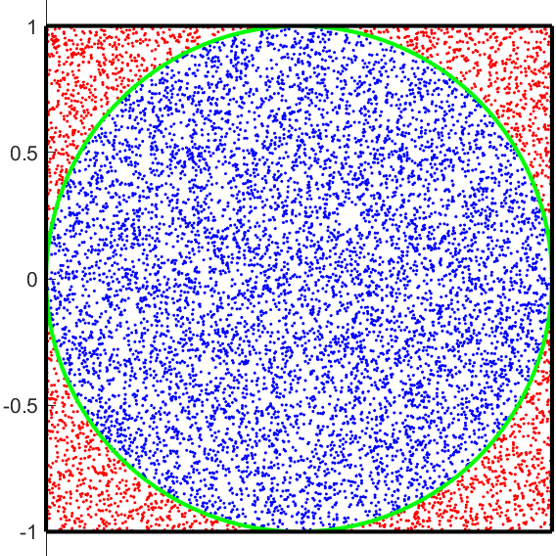
\includegraphics[width=0.5\textwidth]{slika11.png}
\caption{Primer simulacije za iskanje $\pi$}
\end{figure}
\end{frame}

\section{Prikaz varijacijskega grafa}
\begin{frame}
\tableofcontents[currentsection] % Ukaz za vstavljanje kazala
\end{frame}
\begin{frame}
\begin{figure}
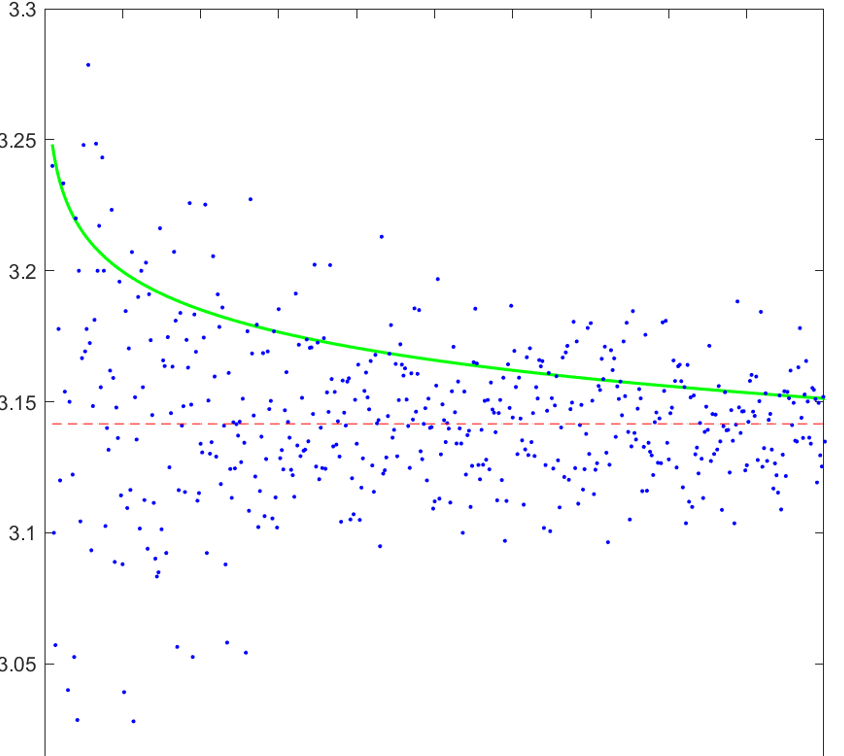
\includegraphics[width=0.7\textwidth]{slika22.png}
\caption{Varijacija naklučno izbranih točk}
\end{figure}
\end{frame}


\end{document}
